%*----------- SLIDE -------------------------------------------------------------
\begin{frame}[t]{Carla Simulator} 
        \begin{columns}[t]
            \column{.5\linewidth}
                \begin{figure}
                    
\includegraphics[trim = 0 0 0 0, clip, width=1\textwidth]{carla.jpg}
                    %\caption{.}
                \end{figure}
            \column{.5\linewidth}
                \vspace*{0.8cm}
                \large{
                \begin{itemize}
                    \item Simulador open-source
                    \item Suporte para desenvolvimento de veículos autônomos
                    \item Integração com ROS
                    \item Pyhton
                    \item GPU com 6 GB necessária
                \end{itemize}
                }
        \end{columns}
%*----------- notes
    \note[item]{Notes can help you to remember important information. Turn on the notes option.}
\end{frame}
%-
\begin{frame}[t]{Carla Simulator} 
    \begin{columns}[t]
        \column{.5\linewidth}
            \begin{figure}
                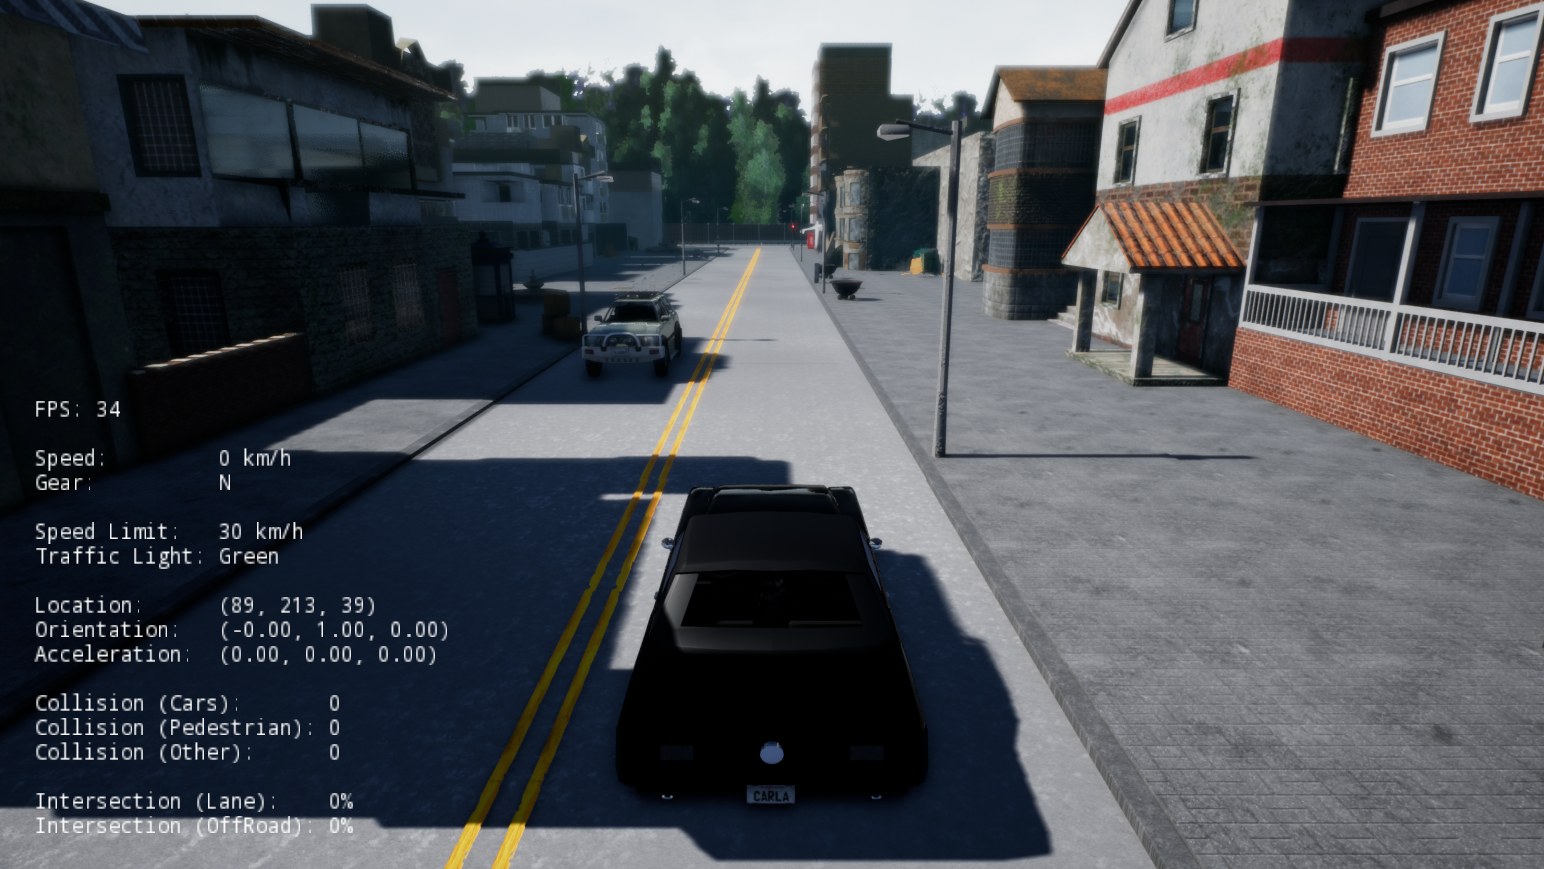
\includegraphics[trim = 0 0 300 0, clip, width=1\textwidth]{simulator_window.png}
                %\caption{.}
            \end{figure}
        \column{.5\linewidth}
            \vspace*{0.8cm}
            \large{
            \begin{itemize}
                \item Carros, pedestres, ambientes urbanos e estradas implementadas
                \item Controle total da dinâmica dos atuadores, geração dos mapas e do ambiente
                \item Ground truth 
            \end{itemize}
            }
    \end{columns}
%*----------- notes
\note[item]{Notes can help you to remember important information. Turn on the notes option.}
\end{frame}
%-
{
\setbeamertemplate{background}
{
\includegraphics[trim = 0 0 0 0, clip, width = \the\paperwidth, height = \the\paperheight]{black.jpeg}}
%*----------- SLIDE -------------------------------------------------------------
\begin{frame}[c]{}
    \transboxout[duration=0.5]
    \begin{center}
    
        \includemedia[
            width=1\linewidth,
            totalheight=0.59\linewidth,
            activate=pageopen,
            passcontext, 
            %transparent,
            addresource=./Source/movies/carla1cut.mp4,
            flashvars={
            source=./Source/movies/carla1cut.mp4
            &autoPlay=false
            &autoRewind=false
            &loop=true}
            ]{\fbox{
\includegraphics{Source/pictures/black.jpeg}}}{VPlayer.swf}
    \end{center}
    
%*----------- notes
    \note[item]{Notes can help you to remember important information. Turn on the notes option.}
\end{frame}
%*----------- SLIDE -------------------------------------------------------------
\begin{frame}[c]{}
    \transboxout[duration=0.5]
    \begin{center}
    
        \includemedia[
            width=1\linewidth,
            totalheight=0.59\linewidth,
            activate=pageopen,
            passcontext, 
            %transparent,
            addresource=./Source/movies/carla2cut.mp4,
            flashvars={
            source=./Source/movies/carla2cut.mp4
            &autoPlay=false
            &autoRewind=true
            &loop=true}
            ]{\fbox{
\includegraphics{Source/pictures/black.jpeg}}}{VPlayer.swf}
    \end{center}
    
%*----------- notes
    \note[item]{Notes can help you to remember important information. Turn on the notes option.}
\end{frame}
}
